%%%%%%%%%%%%%%%%%%%%%%%%%%%%%%%%%%%%%%%%%%%%%%%%%%%%%%%%%%%%%%%%%%%%%%%%%%%%%%%
% Chapter 3: Tecnologías
%%%%%%%%%%%%%%%%%%%%%%%%%%%%%%%%%%%%%%%%%%%%%%%%%%%%%%%%%%%%%%%%%%%%%%%%%%%%%%%

%++++++++++++++++++++++++++++++++++++++++++++++++++++++++++++++++++++++++++++++
\section{Lenguaje para la lógica de la aplicación}
\label{3:sec1}
Por normal general cuando se habla de programación web en el lado del cliente, se tiende a pensar
de forma inmediata en Javascript, y en general, este razonamiento es indudablemente válido. 
Pero dado que SIMDE es una aplicación fuertemente orientada a objetos y con una gran base de código, 
se han valorado múltiples alternativas con el objetivo de agilizar la realización de este proyecto.

\subsection{Coffescript}

Coffescript es un pequeño lenguaje que se compila en Javascript, su objetivo era mejorar la legibilidad 
y concisión de Javascript añadiendo varios \textit{syntactic sugars} inspirados en otros lenguajes como
\textit{Ruby} o \textit{Python}.

\bigskip
Coffescript es un lenguaje con un largo recorrido, apareciendo a finales del año 2009. Y tiene soporte por
parte de \textit{Ruby on Rails} y \textit{Play framework}.

\bigskip 
Coffescript podría ser la opción ideal para agilizar le desarrollo debido a la similitud de sintaxis con 
Ruby.

\begin{lstlisting}
class Animal
  constructor: (@name) ->

  alive: ->
    false

class Parrot extends Animal
  constructor: ->
    super("Parrot")

  dead: ->
    not @alive()
\end{lstlisting}

\bigskip
Sin embargo, la opción de Coffescript ha sido desestimada en gran medida por su decreciente popularidad
y la poca certeza del futuro que tomará el lenguaje.

\subsection{Dart}

Dart es un lenguaje de código abierto desarrollado por Google que permite desarrollador aplicaciones web, móvil, 
de servidor y también se puede utilizar en el \textit{Internet of Things}. 

\bigskip
Se ha considerado en el desarrollo de esta aplicación porque es un lenguaje orientado a objetos que utiliza una 
sintaxis similar a C\#. Además, aunque Google Chrome tiene una máquina virtual nativa para este lenguaje, es posible
transpilar el código a Javascript para los navegadores que no tiene este soporte nativo.

\bigskip
Tras razonar detenidamente, ha pesar de lo atractivo del lenguaje, Dart ha quedado descartado por 
una razón de peso y es que se trata de un lenguaje totalmente diferente y su uso es mayoritariamente
por parte de Google.

\subsection{Typescript}

Typescript es un lenguaje libre y de código abierto desarrollado por Microsoft que actúa como un superconjunto
de Javascript, es decir incorpora los distintos estándares: ECMA5, ECMA6, ECMA7... Y además, como característica
destacable, añade comprobación de tipos en tiempo de compilación.

\bigskip
Este tipado no se refleja en el código final, de hecho una interfaz, por ejemplo,
añade 0 sobrecarga en el código final. Pero si que es interesante por las capacidades de
autocompletado (a través de Microsoft Intellisense)  que añade.

\begin{figure}[!th]
\begin{center}
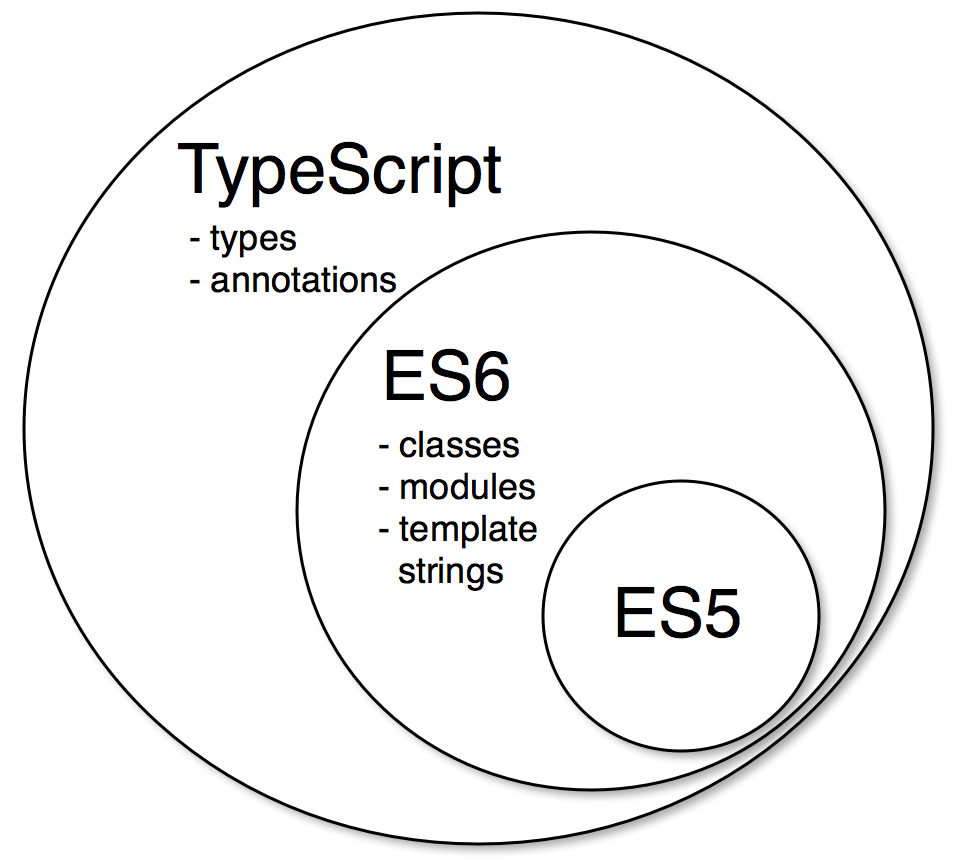
\includegraphics[width=0.5\textwidth]{images/cap3/typescript.eps}
\caption{Typescript como superconunto de Javascript}
\label{fig:Typescript como superconunto de Javascript}
\end{center}
\end{figure}

\bigskip
Al final, en este proyecto Typescript ha sido la tecnología ganadora, y existen múltiples
razones:

\begin{enumerate}

\item Typescript tiene bastante apoyo por parte de la comunidad y por parte de la propia Microsoft.
La documentación es extensa y efectiva.

\item Typescript está alineada en cierta forma con el futuro de Javascript. Microsoft es uno de los 
muchos que forman parate del concenso de estándar de ECMASCRIPT.

\item Typescript no me limita en la posibilidad de usar javascript, todo código javascript es código
Typescript válido.

\item Por último y no menos importante: Tengo experiencia con Typescript.
\end{enumerate}



%++++++++++++++++++++++++++++++++++++++++++++++++++++++++++++++++++++++++++++++
\section{Tecnología para la integración modelo vista}
\label{3:sec2}
Desde el inicio del proyecto, se tenía claro que alguna librería se encargaría de realizar 
por mí el tedioso proceso de manipular el DOM. Actualmente existen múltiples librerías 
y frameworks que podían servir para realizar esta tarea, pero muchos de ellos (como por ejemplo Angular),
son demasiado \textit{"rígidos"} y acaban condicionando la forma de desarrollar la aplicación, 
lo cual resulta ser contraproducente.

\subsection{Webcomponents}

\bigskip
Lo que la nueva versión de SIMDE necesitaba era aprovechar las características que ofrecen los
\textit\textbf{Web Components}. Los Web Components son un conjunto de caracteŕisticas que se 
están añadiendo a las especificaciones W3C de Html y del DOM.

\bigskip 
El objetivo de estas características es permitir crear componentes personalizados, reusables y 
con su propia encapsulación. Esto se consigue a través de cuatro características principales:

\begin{enumerate}

\item \textbf{Elementos personalizados}: Esta característica permite diseñar y utilizar nuevos tipos 
de elementos del DOM.
\item \textbf{Shadow DOM}: Esta característica permite al navegador incluir un subarbol de elementos del 
DOM en el renderizado del documento pero \textbf{NO} se incluyen el DOM principal.
\item \textbf{HTML Imports}: Esta característica permite incluir y reutilizar documentos HTML en otros 
documentos HTML.
\item \textbf{Plantillas HTML}: Esta característica permite declarar fragmentos de código de marcas que no
se utilizan en el carga de la página pero que se pueden instanciar en tiempo de ejecución. 

\end{enumerate}

\subsection{Polymer}
La primera librería que apareció haciendo uso de los Web Components fue Polymer. Polymer es desarrollada por
Google y apareció en el año 2013.

\bigskip
Polymer permitía aprovechar las características de los Web Components a traves de polyfills -los polyfills son
códigos que implementan características en navegadores que no soportan las mismas de forma nativa-. Comúnmente
se conoce como polyfill a la librería que implementa el éstandar de HTML5.

\bigskip
Pero hoy día Polymer no es la única opción disponible, y si tuviera que dar una razón para no utilizar Polymer
es que su comunidad no es tan grande como la de otras librerías y eso acaba traduciéndose en una menor cantidad
de recursos.

\subsection{React}
React es una librería desarrollada por Facebook para construir interfaces.

\bigskip
React utiliza un híbrido entre html y javascript denominado jsx, como también tiene soporte para 
Typescript, en este caso utilizamos tsx, y se basa en un “unidirectonial data-flow”. 

\bigskip
Ademas React implementa operaciones sobre el DOM virtual de tal forma que las operaciones sobre
el verdadero DOM sean eficientes.

\bigskip
Existen una gran cantidad de motivos para escoger React sobre Polymer: Como por ejemplo, 
que ahora mismo se utiliza en decenas de aplicaciones importantes, como netflix, airbnb, Wallmart… (TODO INCLUIR CITA)

\bigskip
Que la comunidad es impresionantemente activa y cuenta con una gran cantidad de usuarios dispuestos a ayudar, así como cuenta con muchísima documentación y muchísimas implementaciones de librerías de terceros.


%++++++++++++++++++++++++++++++++++++++++++++++++++++++++++++++++++++++++++++++
\section{Tecnología para hacer la build}
\label{3:sec3}
Debido a la complejidad de las aplicaciones web modernas, es necesario 
realizar una serie de pasos intermedios entre el código original y 
el resultado final de la apliación. Para el caso de este proyecto, se debe:

\begin{itemize}

\item Compilar el código typescript a javascript.

\item Compilar el código .tsx a .jsx.

\item Resolver las importaciones de dependencias, tanto de la lógica
como de los componentes.

\item Procesar el código sass y convertirlo en css.

\end{itemize}

\subsection{Gulp/Grunt}

La primera tendencia -debido a su gran extensión- sería utilizar 
lo que se conoce como un \textit{task runner}. Actualmente, dos de los 
más conocidos son \textbf{Gulp} y \textbf{Grunt}.

\bigskip
Ambos están basados en NodeJs y son compatibles entre sí en gran medida.
Su funcionamiento es sencillo, en un gruntfile o gulpfile se definen las tareas a
ejecutar, seleccionando los ficheros de fuente sobre los que actuar -si cabe- y la tarea 
a realizar.

\bigskip
Existen muchisimos plugins desarrollados que permiten hacer todo tipo de tareas, desde traducir
markdown hasta minimizar el contenido de los ficheros de estilos y de javascript.

\bigskip
Sin embargo, a pesar de que esta opción era altamente atractiva debido 
a su robustez, se ha optado por probar una solución aún más moderna, \textbf{webpack}.

\subsection{Webpack}

Webpack es un module bundler para aplicaciones de Javascript modernas.
Cuando webpack procesa la aplicación, construye un grafo de dependencias
incluyendo todos los módulos.

\bigskip 
El funcionamiento de webpack puede ser toscamente resumido en:

\begin{itemize}

\item Partiendo de un punto de entrada, una serie de reglas activan una serie de loaders
para procesar los distintos tipos de ficheros. 

\item Para el caso de tareas algo más personalizadas y/o complejas, se utilizan plugins especificos.

\end{itemize}

Como resultado final se obtiene una serie de paquetes que contienen todas las dependencias. +

\bigskip 


%++++++++++++++++++++++++++++++++++++++++++++++++++++++++++++++++++++++++++++++
\section{Tecnología para la documentación}
\label{3:sec4}
Para integrar la documentación en la nueva aplicación web de SIMDE resultaba obvio que esta documentación
estuviera también en formato web. Para esto existían muchas alternativas, desde un conjunto de ficheros
html hasta un pequeño cms. 

Dado que la documentación es bastante extensa pero que en realidad, no es mas que un documento 
que se redactará en una ocasión y se le irán realizando pequeñas ampliaciones y/o correcciones
se optó por una solución diferente, los generadores de contenido estático.

\subsection{Generadores de contenido estático}

Los generadores de contenido estático se encargan -resumido de forma tosca y breve- de generar 
un conjunto de htmls y css a partir de una plantilla y una serie de ficheros fuentes. 

\bigskip
Este tipo de generadores estáticos tienen un gran auge entre los desarrolladores que desean 
mantneer un blog -yo mismo por ejemplo, tengo uno hecho en Hugo-. 

\bigskip 
Existen múltiples ventajas de utilizar este tipo de tecnologías, pero sin duda para mi la más
importante, es que se alimentan de un formato como es el markdown. El cual es muy intuitivo de 
usar y tiene soporte más allá de este tipo de tecnologías. 

\subsection{Hexo}

Hexo es un generador de contenido estático basado en NodeJS. No posee demasiadas diferencias destacables
sobre el resto y ha sido escogido para este trabajo de fin de grado básicamente por estar basado 
también en Javascript, de tal forma que todo quede enfocado hacia javascript.

\bigskip
¿Comparativa hexo vs jekyll vs hugo?
